\section{Introduction}\label{sec:introduction}

In today's fast-moving software world, no large software project is developed by
one single person. Team coordination becomes a challenging factor in software
development, as success rates drop with increasing team sizes
\cite{ambler:2010}. Another central pillar of modern software development is
testing. While proper software testing clearly boosts software quality, it can
be incredibly expensive \cite{dustin:1999}.\\

Continuous Integration is an approach to addresses these problems by
\begin{enumerate}[label=(\alph*)]
    \item Applying small incremental changes over time to a central source code
       repository
    \item Employing an automated testing strategy
\end{enumerate}

and strives to improve team efficiency all together.

\subsection{History}\label{sec:history}

Before Continuous Integration, developers worked on their own separate copies of
the project for (possibly) long amounts of time. The integration phase of
software development was scheduled at the end of feature implementation. The
problem here is, that not all developers worked on the same setup. They use
different tools or versions on different machines. This would cause various
instances of "works-for-me"-bugs, issues that appeared for some, but not for all
involved individuals.\\

To prevent this from happening (at least for build-time-errors), often a
designated build-machine was employed - a server that developers pushed their
commits to that would automatically build the whole project. Commits would only
be considered valid if the build-server was able to build them. Various tools
were developed to run on these servers (see \ref{sec:tooling-self-hosted}) and
gradually, these server's capabilities were expanded beyond just building
\cite{zilberfeld:2013}.\\

When Continuous Integration first became popular, it was tightly coupled to many
concepts practiced in Extreme Programming. In this software development
methodology, (typically small) development teams use various coding-focused
techniques in order to develop software faster.

\subsection{Motivation}\label{sec:motivation}

The main goal of Continuous Integration is to minimize integration issues when
deploying release-versions of the product. Because builds happen often and
regularly, these issues can be identified very quickly and will not cause
stressful last-minute fixes. The incorporation of unit tests into the
build (see \ref{sec:testing}) can further accelerate error detection. Another
important aspect of Continuous Integration is the provision of a reporting
agent, a way that developers get informed about failing builds.

\subsubsection{Merge hell}\label{sec:merge-hell}

In big software projects, a large number of developers work together to create
software. To be able to work on the same project simultaneously, typically, a
version-control system such as GIT is utilized
\footnote{\url{http://git-scm.com/}}.\\

Developers usually branch off from a common baseline ("master"), implement their
feature in their own copy ("feature-branch") and when finished, merge their
branch back into the master. However, if a large number of developers do that
and their features are large and/or implemented in overlapping parts of the
source code, developers have to face merge-conflicts when integrating their
branch back into the baseline. These conflicts can easily get out of hand.
Figure \ref{fig:merge-hell} shows an example of such a situation.

\begin{figure}[h]
    \centering
    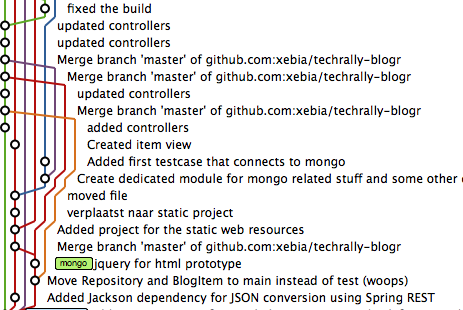
\includegraphics[width=0.6\linewidth]{images/merge-hell.png}
    \caption{An example of "merge-hell" \cite{mooij:2010}}
    \label{fig:merge-hell}
\end{figure}

Solving these conflicts can be non-trivial task, especially for the introduction
of completely new features, since the developer who has to perform the merge
typically is not yet accustomed to the code another developer only just
created.\\

In order to keep large merge conflicts to a minimum and therefore circumvent
this issue, Continuous Integration strives to integrate features back into the
baseline branch frequently (e.g. multiple times per day).  Of course, this means
that the term "feature" is bound to refer only to small changes throughout the
project's life cycle.
